\documentclass[exercice]{thedocument}%
\usepackage{texmaths-tikz}%
\startdatakeys
\source{}
\cycle{}
\competencesDuSocle{}
\connaissancesRequises{}
\competencesTravaillees{}
\enddatakeys
\begin{document}%
\begin{enumerate}
    \item Écrire une expression littérale donnant le {\bfseries périmètre} du rectangle ABCD.
    \item Écrire une expression littérale donnant l'{\bfseries aire} du rectangle ABCD.
\end{enumerate}
\begin{center}
    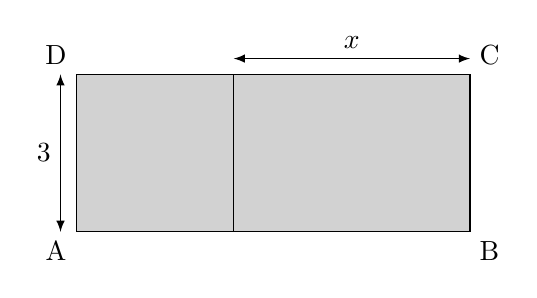
\begin{tikzpicture}
        \coordinate[label=below left:A](A)at(0,0);
        \coordinate(B)at(2,0);
        \coordinate[label=below right:B](C)at(5,0);
        \coordinate[label=above right:C](D)at(5,2);
        \coordinate(E)at(2,2);
        \coordinate[label=above left:D](F)at(0,2);
        \path(D)+(0,0.2)coordinate(D1);
        \path(E)+(0,0.2)coordinate(E1);
        \path(F)+(-0.2,0)coordinate(F1);
        \path(A)+(-0.2,0)coordinate(A1);
        \draw[fill=gray!35](A)rectangle(D);
        \draw(B)--(E);
        \draw[latex-latex](D1)--(E1);
        \path(D1)--(E1)node[midway,above]{$x$};
        \draw[latex-latex](A1)--(F1);
        \path(A1)--(F1)node[midway,left]{$3$};
        \tkzMarkRightAngle(B,C,D)
        \tkzMarkRightAngle(C,D,E)
        \tkzMarkRightAngle(B,E,F)
        \tkzMarkRightAngle(E,F,A)
        \tkzMarkRightAngle(F,A,B)
        \tkzMarkRightAngle(A,B,E)
        \tkzMarkSegments[mark=s||](E,F F,A)
    \end{tikzpicture}
\end{center}
\end{document}
